\section{Story Diagrams} \label{sec:StoryDiagrams}

\subsection{General Idea (Dietrich)}

% - combine activity diagrams and graph transformations as well as imperative, deterministic and declarative, non-deterministic languages to formally and compactly describe software behavior in terms of model transformations using an OO-based, familiar notation

The main idea behind story diagrams is to formalize UML activity diagrams
to better support model-driven software development
by means of completely modeling software structure and behavior and making the software model executable.
For that purpose, graph transformations, a well-known formalism, were chosen to formally specify behavior and have been combined with UML activity diagrams.
The result, story diagrams, is a mixture of two languages:
an imperative, deterministic language for the description of control flow, UML activity diagrams,
and a declarative, non-deterministic, object-oriented, graph-transformation-based language for the description of model modifications, so-called story patterns (see Section~\ref{sec:StoryPatterns}).
Both languages are graphical, formally defined, and use a familiar notation based on UML 1.5 activity diagrams and UML object diagrams with minor modifications.

An exemplary story diagram is illustrated in Figure~\ref{fig:simpleStoryDiagram}.
This story diagram replaces calls of a given method (\emph{oldMethod}) with calls of another given method (\emph{newMethod}).

\begin{figure}[htb]
  \centering
  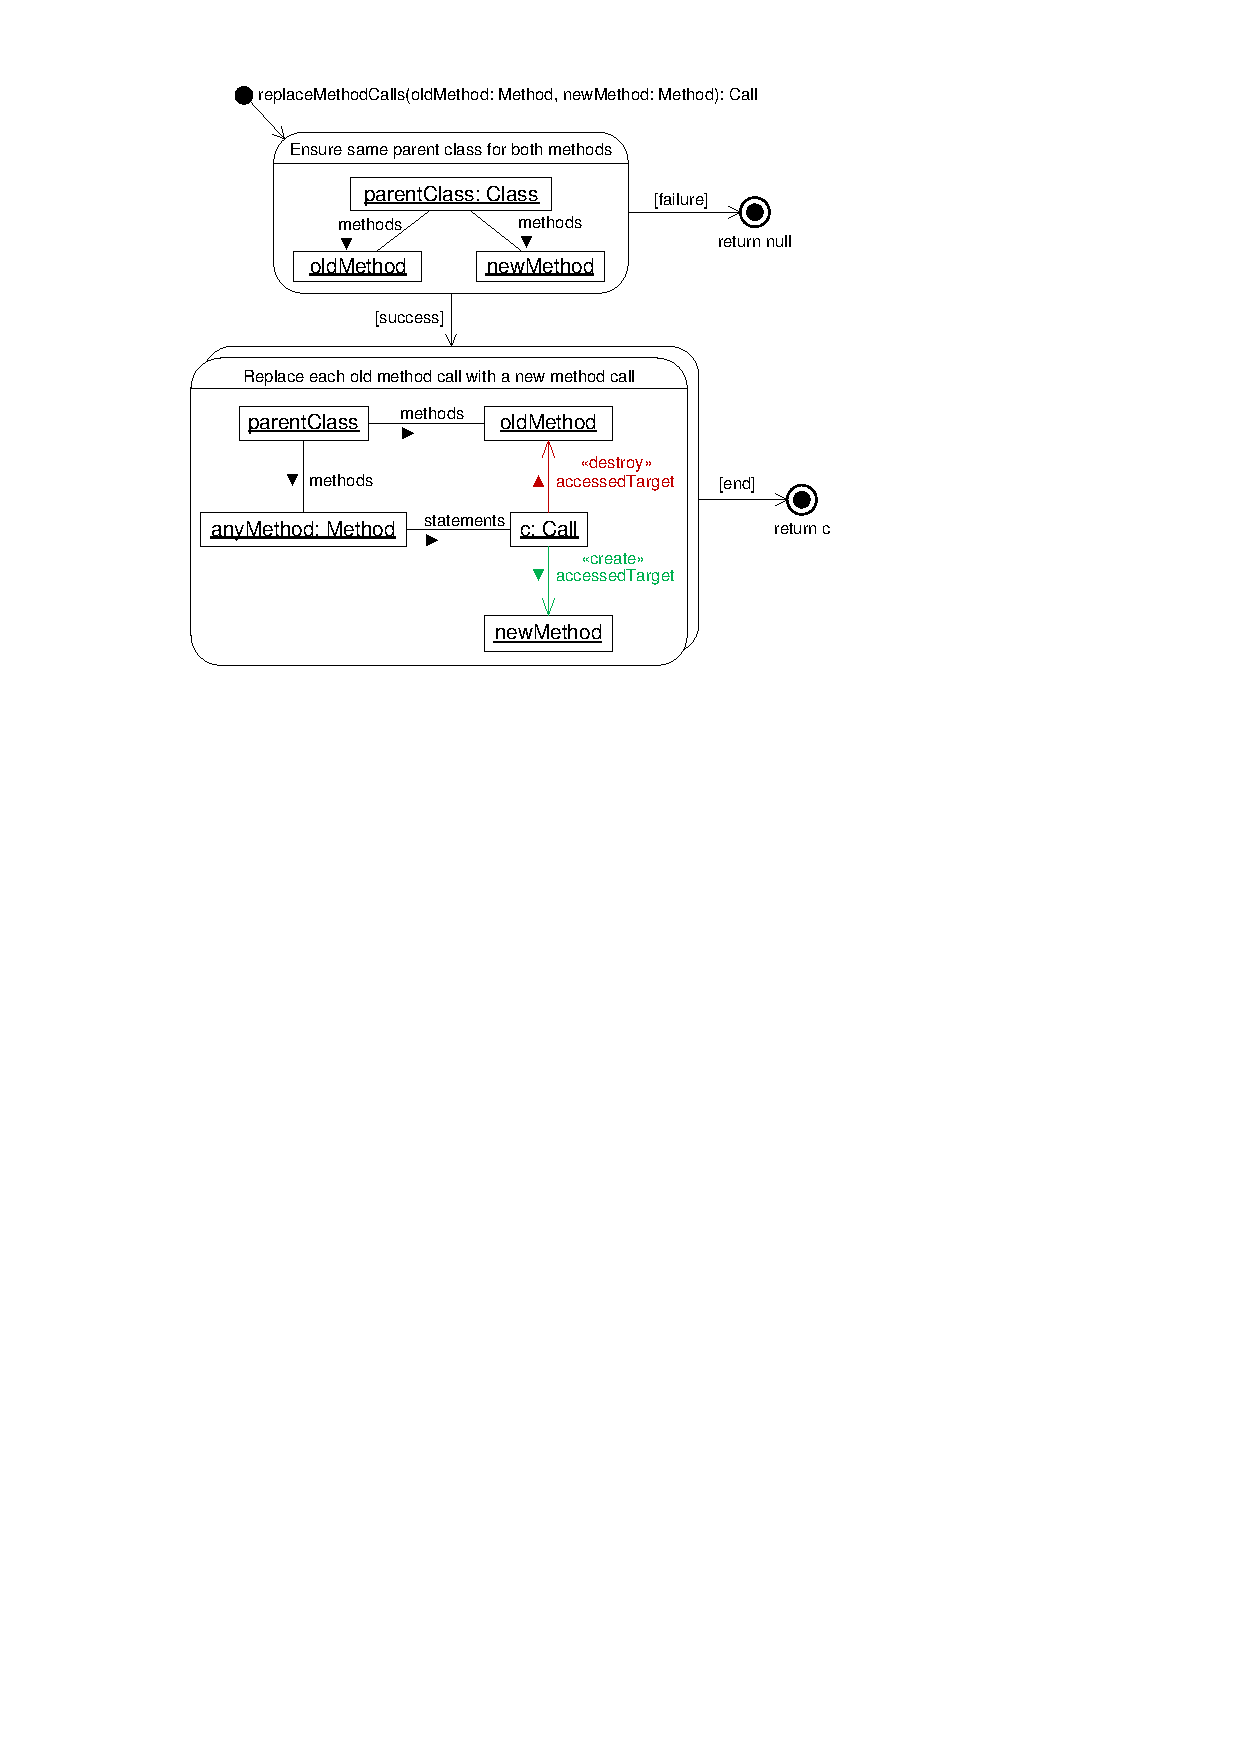
\includegraphics[scale=1.0]{figures/SimpleStoryDiagramExample}
  \caption{Exemplary Story Diagram -- Replace Method Calls}
  \label{fig:simpleStoryDiagram}
\end{figure}

Like UML activity diagrams, story diagrams model control flow by means of activity nodes and activity edges.
Each activity node contains a story pattern to formally specify the behavior for this node\footnote{There are
some few exceptions like activity call nodes which do not contain story patterns to specify the behavior.}.
The activity edges can carry guards.
These are either boolean expressions, e.g., checking attribute values of a matched object,
or guards used to specify decisions on whether a story pattern could be
matched or not\footnote{A story pattern is successfully matched if for each object and link variable in the pattern corresponding objects and links are found in the instance model (host graph) and all specified constraints are satisfied.}.
In Figure~\ref{fig:simpleStoryDiagram} the used guards are \text[success\text] (successful matching),
\text[failure\text] (failed to completely execute a story pattern),
and \text[end\text] (activity edge points to the first activity node to be executed after a loop).

In contrast to ordinary UML activity diagrams, story diagrams, so far, do not model concurrent execution.
Thus, the language constructs \emph{fork} and \emph{join} are omitted in story diagrams.

%- Story diagrams in MDSD process, 2 worlds: stand-alone transformations and specifications of methods' behavior:
%  1. alternative (completely modeling software): model classes in class diagrams, specify their methods' behavior in story diagrams, generate executable source code (e.g. Java) or use an interpreter
%  2. alternative (specify recurring model operations/transformations for a given type of models): model only classes representing the editor's model under development (meta-model), specify modification operations of this model (adding and removing elements, analysis operations, translations to/generation of other models, etc.), need of a software that triggers the specified operations, the operations can be performed using generated code or an interpreter
%- introduce an example

Basically, there are two slightly different ways of using story diagrams in a model-driven software development process.

Originally, story diagrams were used in object-oriented software development to formally specify the behavior of methods that are defined in classes.
Calling such a method means to execute the story diagram that represents the method's behavior.
If for all defined methods story diagrams are specified, the software can be executed.
In this case, story diagrams specify the behavior of objects whose properties are defined by classes.
Thus, story diagrams have a \emph{this} variable representing an object (class instance) that they belong to.
This variable can be used as a starting point for the graph matching specified in a story diagram.

For example, the class diagram in Figure~\ref{fig:SDWithThisClassDiagram} defines a method \fe{findAttribute} for all \fe{Class} objects.
This method's behavior is specified by the story diagram in Figure~\ref{fig:SDWithThis}.
The matching of the object structure specified in the story diagram, in this case,
starts with the \fe{this} object variable of the type \fe{Class} which is already bound
to the \fe{Class} object that the \fe{findAttribute} method belongs to.
Thus, this method tries to find an attribute \fe{a} in the same class with the name given by the method's parameter \fe{text}.

\begin{figure}[tb]
	\centering
  \begin{minipage}[t]{.4\textwidth}
    \centering
    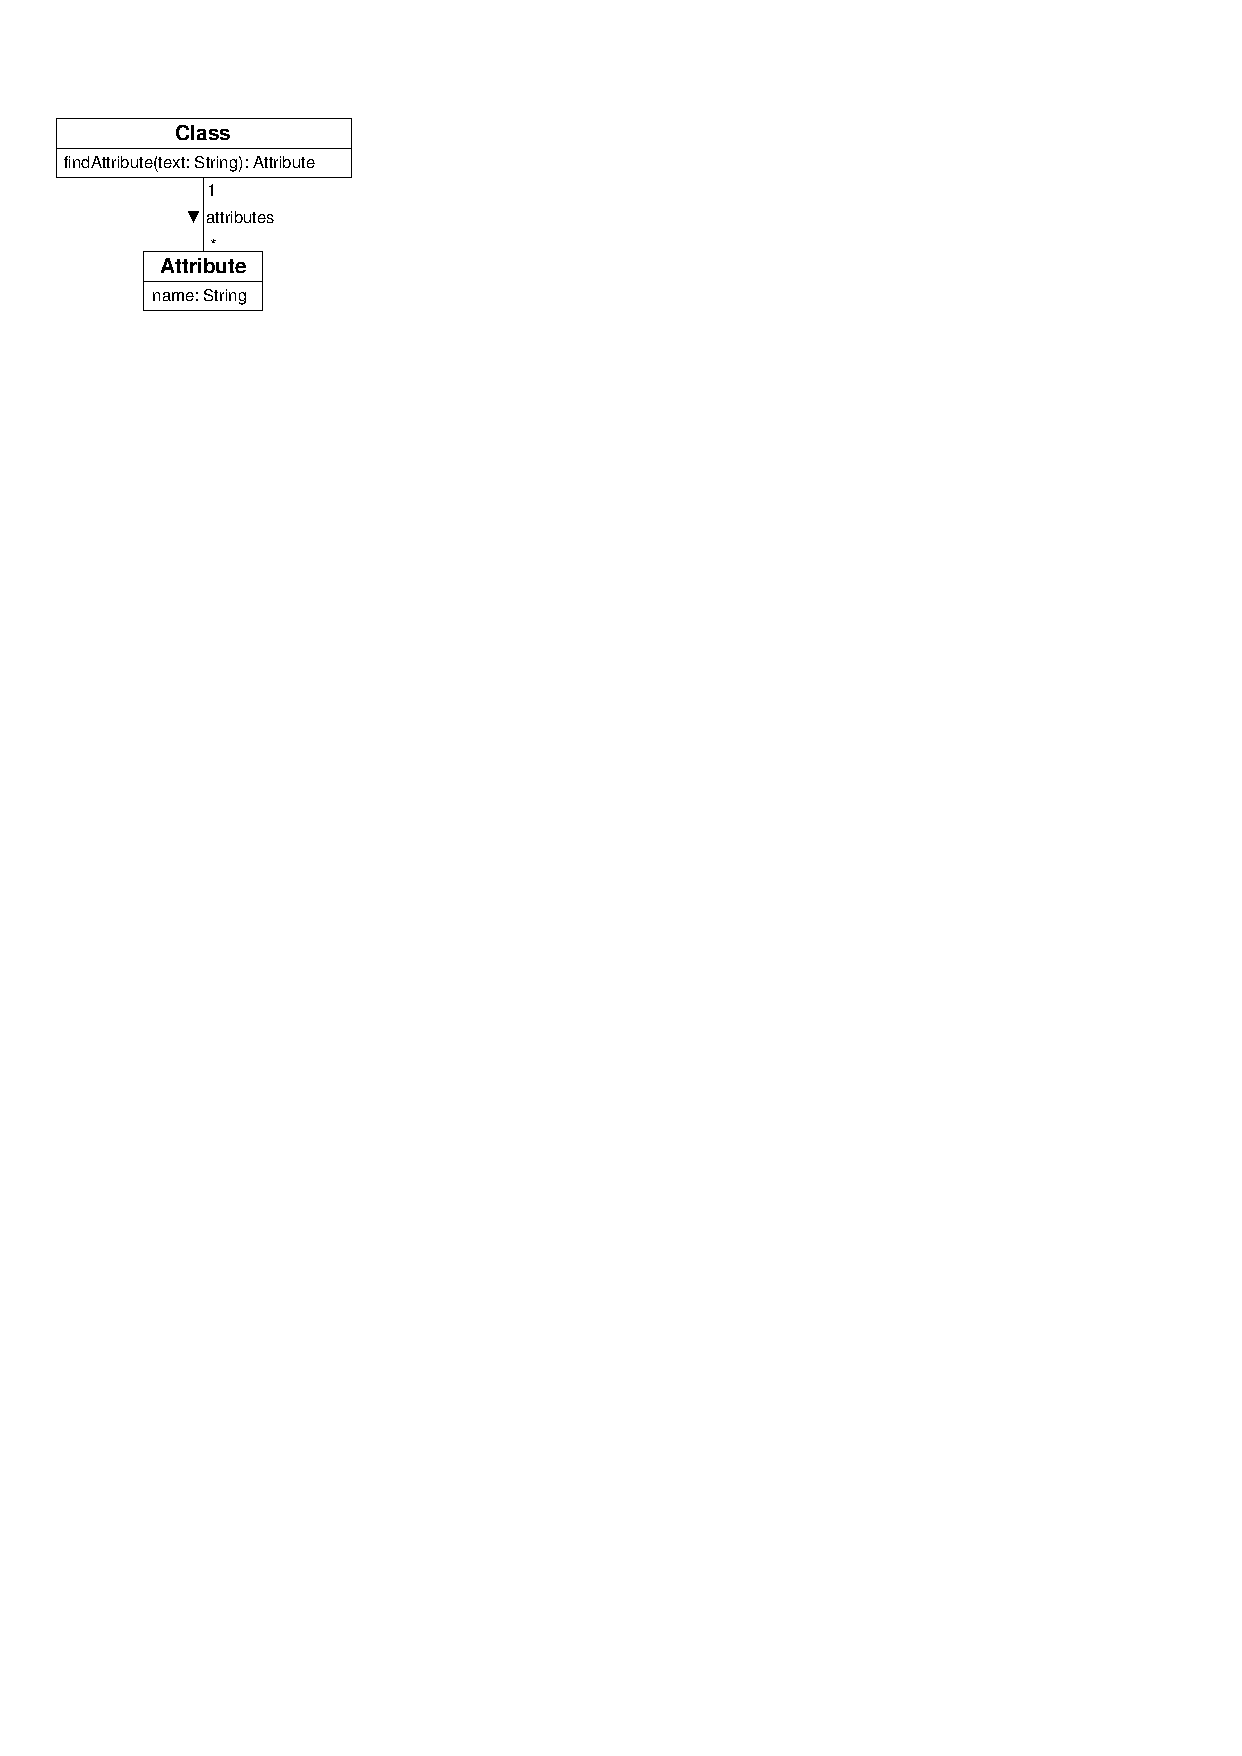
\includegraphics[scale=1]{SimpleSDFindAttributeClassDiagram} 
    \caption{Type Model for the Story Diagram in Figure~\ref{fig:SDWithThis}}
    \label{fig:SDWithThisClassDiagram}
  \end{minipage}%
  \hfill
  \begin{minipage}[t]{.55\textwidth}
    \centering
    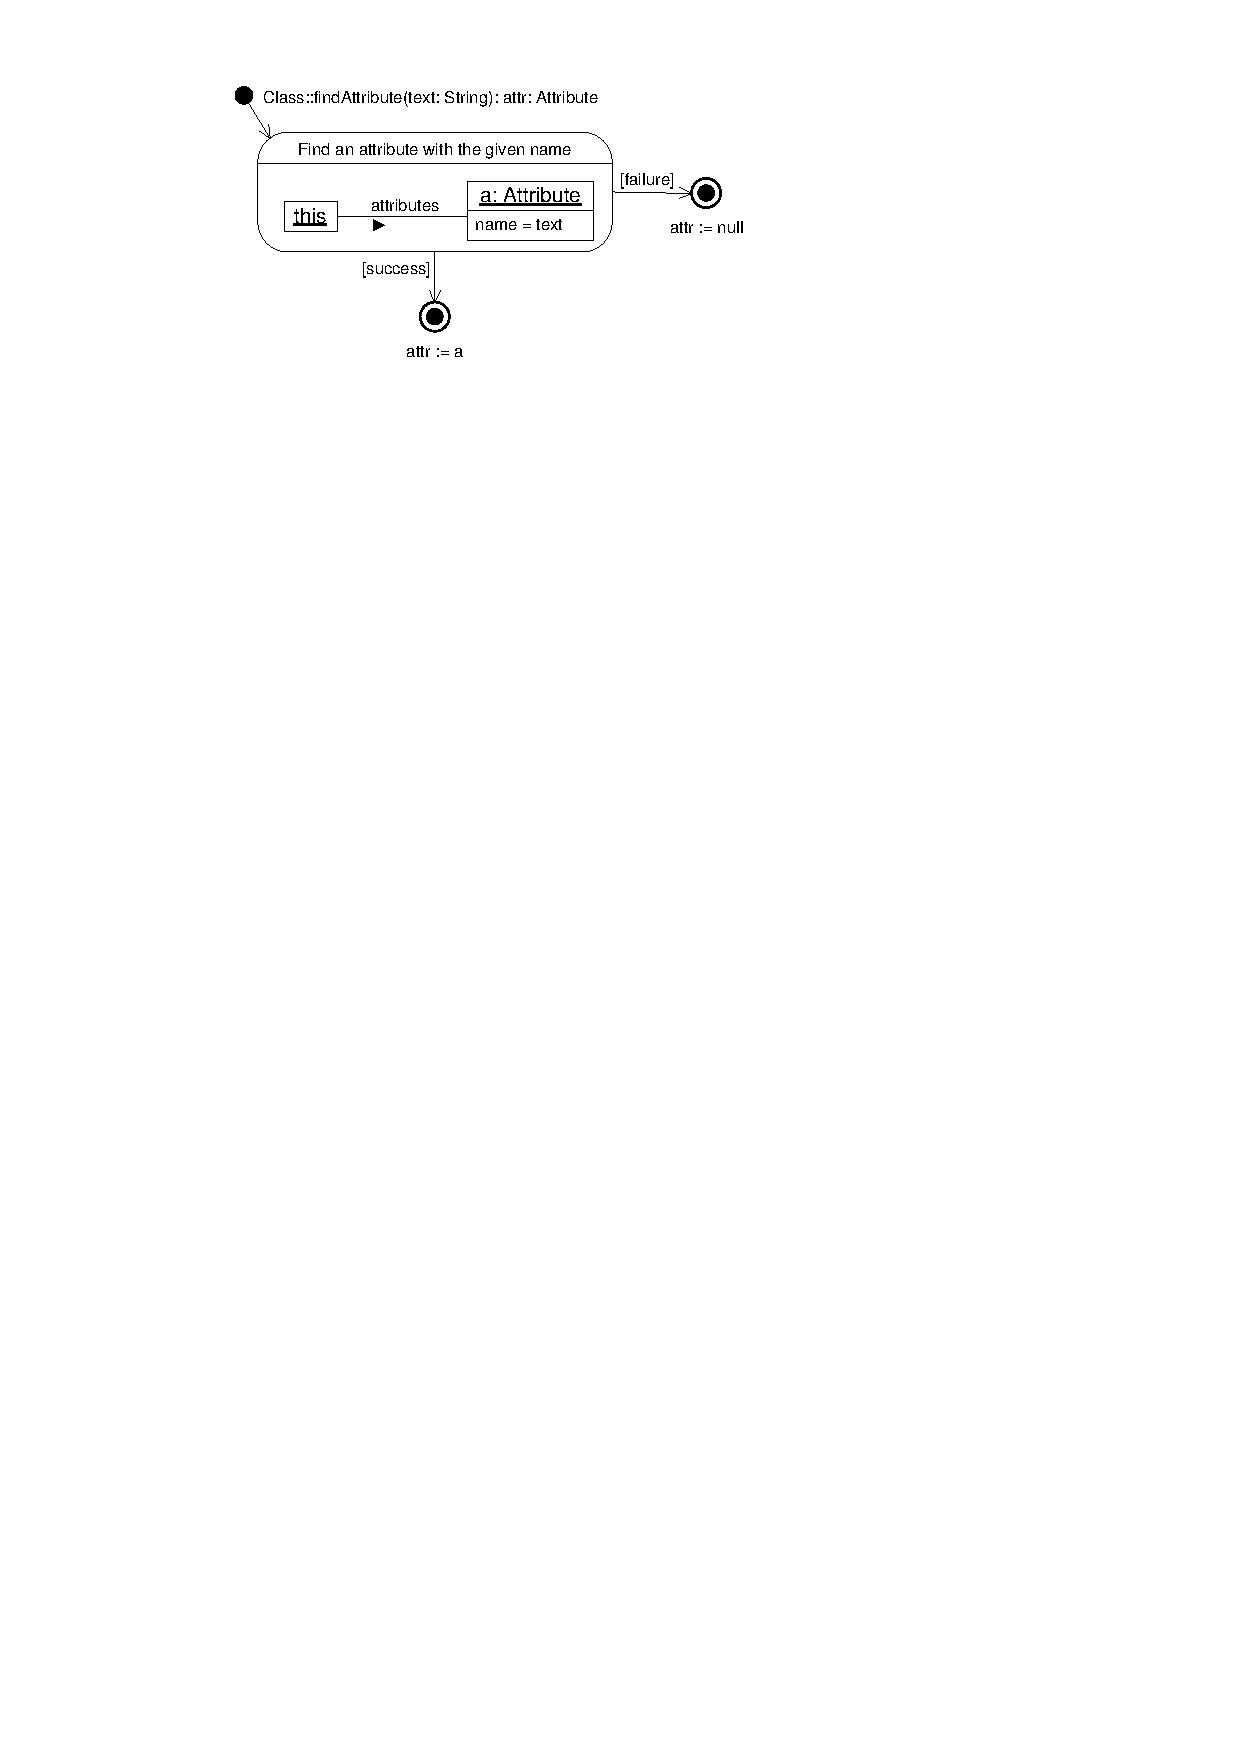
\includegraphics[scale=1]{SimpleSDFindAttribute}
    \caption{Exemplary Story Diagram With \emph{this} Object Variable}
    \label{fig:SDWithThis}
  \end{minipage}
\end{figure}

\begin{figure}[tb]
	\centering
  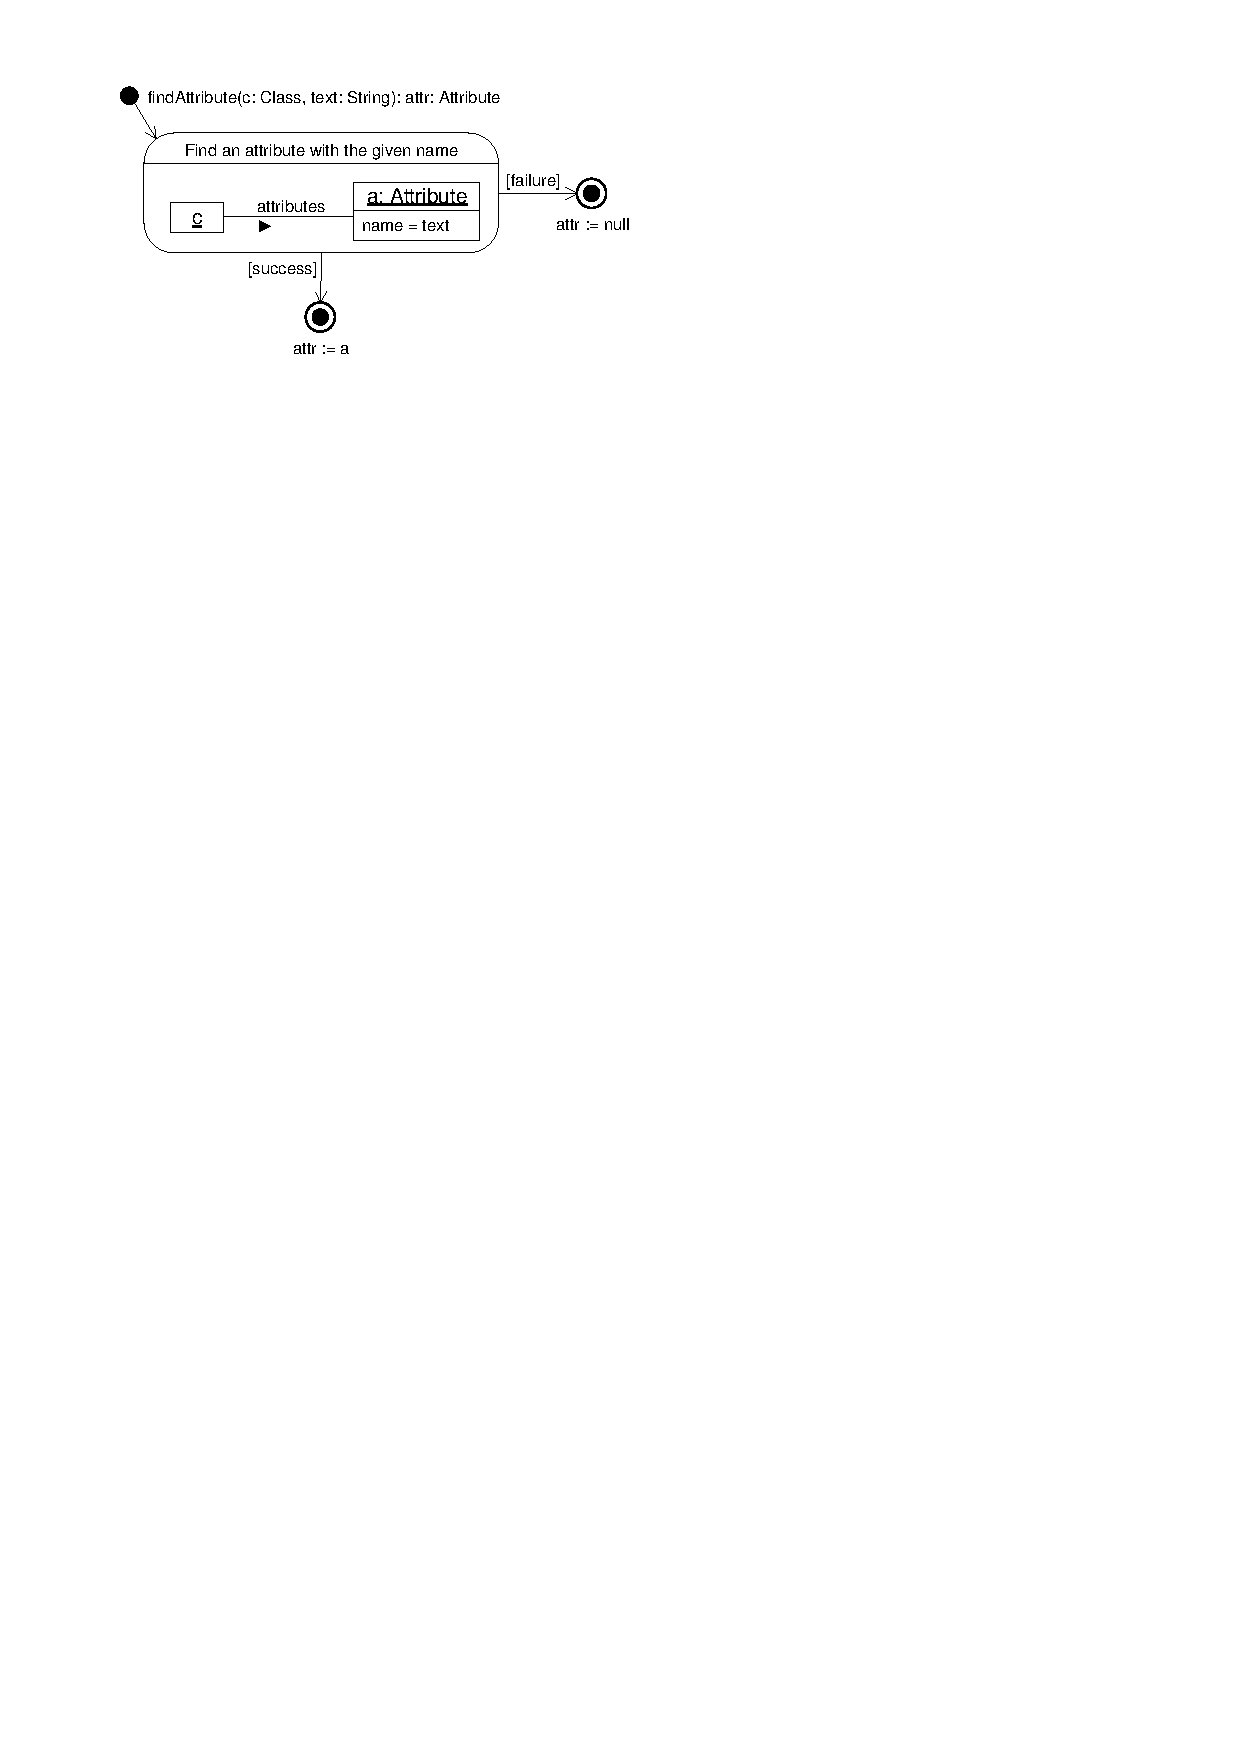
\includegraphics[scale=1]{SimpleSDFindAttributeStatic} 
  \caption{Exemplary Story Diagram Without \emph{this} Object Variable}
  \label{fig:SDWithThisStatic}
\end{figure}

Another more flexible way of using story diagrams is to specify any kind of model transformation or operation in a story diagram without sticking this behavior to a certain class.
In contrast to the previous case, there is no \emph{this} variable that could be used as a starting point for the graph matching.
All starting nodes for the graph matching have to be provided as arguments of the story diagram call.
For this purpose, in contrast to the story diagram in Figure~\ref{fig:SDWithThis}, the story diagram in Figure~\ref{fig:SDWithThisStatic} has an additional parameter \fe{c}.
The corresponding arguments of a story diagram call are assumed to be known (bound object variables) and are used as starting points for the graph matching.
This way, the operations or transformations defined by story diagrams can be used from within any other part of the developed software, like a software library would be used.
Typically, model-to-model transformations, consistency checks, or more generally speaking, recurring and object-independent operations are defined this way.

% - enable formal analyses to check/ensure certain behavioral software properties

In both cases the story diagrams can be used to generate executable source code or be executed using an interpreter.
Besides execution, the formally defined story diagrams can also be analyzed to guarantee certain behavioral properties.
For example, model checking can be used to check if a certain invariant holds
(e.g.\ all accessible variables are still accessible after refactoring operations)
or if a critical state can ever be reached (e.g.\ attributes or methods having no parent class after refactoring operations).

A complete description of the story diagrams' abstract syntax is given in the Appendix~\ref{sec-reference}.
There is also a grammar that determines all feasible story diagrams by constraining their structure.
The last published version of this grammar can be found in Thomas Klein's diploma thesis \cite{Kle99}.


%\subsection{The Language Constructs in Story Diagrams (Jan/Dietrich)}\label{sec:StoryDiagrams:composition}

\subsection{Activities, Activity Parameters and Return Values (Dietrich)}

Since story diagrams can be seen as special UML activity diagrams, we reused the class names defined by the UML.
Thus, similar to UML activity diagrams, a story diagram is represented by a so-called activity (class \fe{Activity}).

Each story diagram can have parameters.
We distinguish \emph{in} and \emph{out} parameters,
i.e. parameters representing arguments given when a story diagram is called (\emph{in})
and parameters representing return values (\emph{out}).
Parameters can be \emph{in} and \emph{out} parameters at the same time.
The story diagram in Figure~\ref{fig:SDWithThisStatic} has two \emph{in} parameters \fe{c} and \fe{text}
as well as an unnamed \emph{out} parameter of the type \fe{Attribute}.

If a story diagram defines the behavior of a method, the parameters are defined by the corresponding method's signature.
In this case, the number of \emph{out} parameters is limited to one single parameter and represents the only \emph{return} value of the method and story diagram.
Besides these parameters there is another implicitly defined parameter \emph{this}
which -- similar to Java's \emph{this} keyword -- represents the object that the story diagram belongs to.

In case that a story diagram is not defining a method's behavior, it defines it's own signature explicitly with according \emph{in} and \emph{out} parameters.
The number of \emph{out} parameters is allowed to be arbitrary in this case and there is no \emph{this} parameter.

The values or objects returned after execution of a story diagram are defined by the expressions in the \emph{stop} activity nodes.
For example, the object matched to the object variable \fe{a} is returned by the story diagram in Figure~\ref{fig:SDWithThisStatic} in case of a successful execution.
Otherwise, the \emph{null} reference is returned which is specified by the keyword \emph{null}.


\subsection{Activity Nodes, Activity Edges (Dietrich)}

A story diagram's control flow is defined by activity nodes and activity edges, similar to UML activity diagrams.
Except of a few exceptions where an activity node represents a call of another story diagram,
each node contains a story pattern to specify the corresponding behavior.
Such activity nodes are called \emph{story nodes}.
Executing a story node results in executing the corresponding story pattern.

In contrast to single story patterns, story patterns contained in story nodes of a story diagram have another scope.
Here, you can reuse all object variables declared in a story pattern of a preceding story node.
For example, in Figure~\ref{fig:simpleStoryDiagram} (p.~\pageref{fig:simpleStoryDiagram}),
the object variable \fe{parentClass} is reused in the following story pattern
by specifying the variable as a bound variable
(i.e.\ the variable does not have to be matched anymore, the object matched in the steps before is used instead).

Executing a story node means to execute the corresponding story pattern
which means to find a subgraph with the specified properties
(e.g.\ find objects of a certain type, with certain attribute values, and with certain connections)
and to perform specified modifications of the found subgraph
(e.g.\ creating or removing objects and links or changing their attribute values).

We distinguish two kinds of story nodes: \emph{modifying story nodes} and \emph{matching story nodes}.
A matching story node contains a story pattern that only matches a specified object structure, but does not change it.
A modifying story node is in addition allowed to perform modifications of the matched obejct structure.
For static analyses of graph transformations described with story diagrams it is helpful to know which tranformations do not modify the host graph (instance model).


\subsection{Decision Nodes, Guards, and Loops (Dietrich \& Jan)}

Due to story node behavior being defined by story patterns,
since trying to find a subgraph defined by a story pattern can fail,
each execution of a story node can also fail.
To distinguish the cases of a successful story node execution and its failure,
the outgoing activity edges can be provided with the guards \text[success\text] and \text[failure\text].
The control flow is following the activity edge with the \emph{success} guard in case of a successful story node execution,
i.e.\ a successful matching of the corresponding story pattern,
otherwise it follows the activity edge with the \emph{failure} guard.
If an outgoing activity edge has no guard, it covers both cases, success and failure.
The guards \text[success\text] and \text[failure\text] can only be used pair-wise (exactly two outgoing activity edges with exactly these two guards).
The first story node in Figure~\ref{fig:simpleStoryDiagram} (p.~\pageref{fig:simpleStoryDiagram}) uses these guards.

Besides \text[success\text] and \text[failure\text] boolean expressions can be used as guards.
In this case, after execution of an activity node the boolean expression of the outgoing activity edge is evaluated to \emph{true} or \emph{false}.
There can be arbitrarily many outgoing activity edges with boolean guard expressions,
but the boolean expressions have to mutually exclude each other
and the corresponding guards have to be combined with an outgoing activity edge with the guard \text[else\text],
i.e.\ if there is a guard with a boolean expression, there is also an activity edge with the guard \text[else\text].

\tododt{add a figure for illustration of various boolean guards}

Guards can be used to model loops.
For that purpose we use the guards \text[for each\text] and \text[end\text] in combination which is further explained in the following.
A special story node is the \emph{for-each} activity node, depicted by a cascading activity node.
The second activity node in Figure~\ref{fig:simpleStoryDiagram} is a \emph{for-each} activity node.
Such a node represents a loop where the contained story pattern is executed as often as new subgraphs can be matched
that differ from the previously matched graphs by at least one other matched object.
For example, the story pattern in the \emph{for-each} activity node in Figure~\ref{fig:simpleStoryDiagram}
is matched for each existing pair of a method (object variable \fe{anyMethod}) and corresponding call object (object variable \fe{c}).
Besides the matching itself, all \emph{destroy} and \emph{create} steps are also executed for each of these matched subgraphs.
After all these matching steps, the control flow is guided by the outgoing activity edge with the guard \text[end\text].
Each \emph{for-each} activity node has such an outgoing activity edge.
In addition, this edge can be combined with another activity edge having the guard \text[for each\text].
This edge is leading to the activity node (or e.g.\ a sequence of such nodes)
that is to be executed after each successful execution of the \emph{for-each} activity node.
In this case, there has to be an activity edge leading back to the \emph{for-each} activity node
to terminate the specified loop by following the \text[end\text] activity edge.

\tododt{add a figure for illustration of loops}

\tododt{add a figure for illustration of decision nodes}

\todojr{fresh matches, auch fuer maybe\_bound (Stefan fragen wegen Beispiel)}


\subsection{Story Diagram Calls (Markus)}

Story diagram calls are special nodes in a story diagram which are used to invoke other story diagrams. Similar to method calls, this reduces redundancy and promotes reuse.

As described in the previous sections, a story diagram can have an arbitrary number of in and out parameters. When calling a story diagram, concrete arguments have to be assigned to the in parameters. Consequently, if an object variable named n is bound somewhere in the story diagram, the identifier n can be used to pass this object variable as an argument to a call. Similarly, if the called story diagram has out parameters, those are implicitly bound to their respective names and can be used by specifying object variables of the same name.

In contrast to QVT \cite{QVT}, we do not explicitly model inout parameters. Instead, we allow the same objects which are passed as in parameters to be also returned as out parameters.
These objects are not bound again after the call. Instead the binding is preserved and the same object variable is used before and after the call. This is similar to the semantics of a call-by-reference parameter.

An example of a story diagram call is shown in Figure~\ref{fig:call}.

\begin{figure}[htb]
\begin{center}
  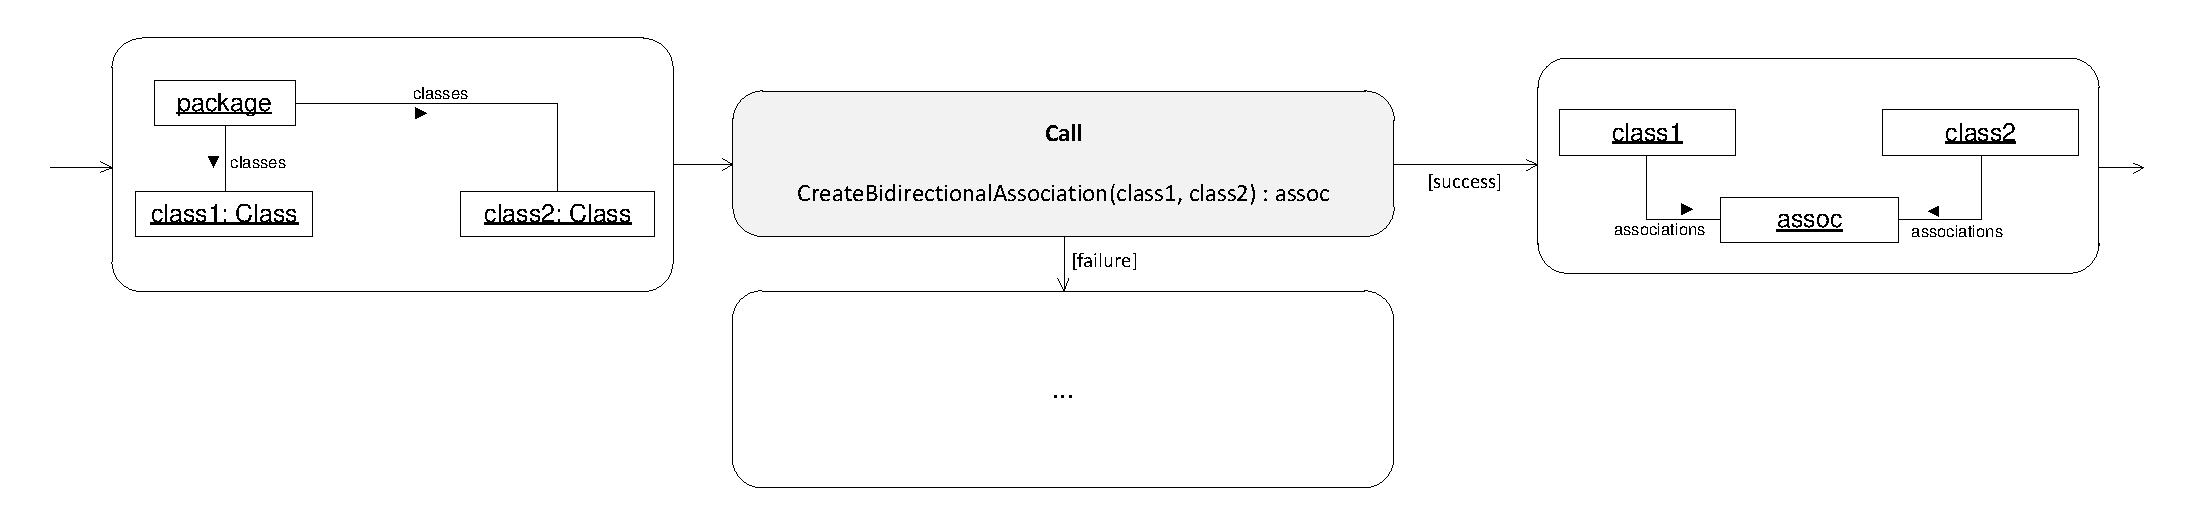
\includegraphics[width=\textwidth]{figures/StoryDiagramCall}
  \caption{Example of a story diagram call}
  \label{fig:call}
\end{center}
\end{figure}

The first story pattern in Figure~\ref{fig:call}, shows the bound object variable \fe{package}. Two new object variables \fe{class1} and \fe{class2} are bound in that pattern. The next node with the grey background is a story diagram call which is also signified by its label. Beneath the label, the name of the called story diagram is given, in this case \fe{CreateBidirectionalAssociation}. Assume that the called story diagram has two in parameters of the type \fe{Class} and one out parameter of the type \fe{Association}. The two classes that were bound in the first story pattern, \fe{class1} and \fe{class2} are passed to the call as arguments.
The result of the call is bound to the object variable \fe{assoc}. The type of this variable is determined by the out parameter type, i.e., in this case the type Association.

If a story diagram has no out parameters, the colon and the out parameters names after the parentheses are omitted (see Figure \ref{fig:SDRemoveInterfaceViolation} for an example).

%Issues for future versions:
% method calls
% polymorphic calls

\ext{
\subsection{Exception Handling (maybe not in Ver. 0.1)}
}


